\section{Lys sensor}
Udgangspunktet for denne undersøgelse er så vidt som muligt at bruge de komponenter vi har til rådighed i Embedded Stock. Hvilket umiddelbart betyder lyssensore af typerne: TEMT6000, TSL2561, og TCS230.

Undersøgelsen har som mål at finde sensorer der (i prioriteret rækkefølge):
\begin{enumerate}
    \item Har gode egenskaber inden for det synlige spektrum (ca. 400 – 700 nm).
    \item Kan tilgås med en interessant protokol – I2C er foretrukket.
    \item Er i stand til at måle farvetemperaturer.
\end{enumerate}

\begin{table}[H] \centering
\begin{tabular}{|p{3cm}|p{11cm}|}
	\hline
	\textbf{Løsning}		
	    & TEMT6000 
	\\ \hline
	\textbf{Producent} 		
	    & Vishay Semiconductors 
	\\ \hline
	\textbf{Interface} 		
	    & Analog output (strøm, typisk: 10-50 $\mu$A) 
	\\ \hline
	\textbf{Beskrivelse} 	
	    & Simpel sensor, der måler lysintensitet 
	\\ \hline
	\textbf{Krav} 			
	    & Opfylder krav 1 
	\\ \hline
	\textbf{Fordele}		
	    & Simpel, fornuftig spektrum responskurve 
	\\ \hline
	\textbf{Ulemper} 		
	    & Lidt for simpel kommunikation, responskurve strækker sig lidt over i det infrarøde område, kan ikke måle farver 
	\\ \hline
	\textbf{Pris} 			
	    & Tilgængelig i Embedded Stock 
	\\ \hline
	\textbf{Link} 			
	    & \url{https://www.sparkfun.com/datasheets/Sensors/Imaging/TEMT6000.pdf} 
	\\ \hline
	\multicolumn{2}{|c|}{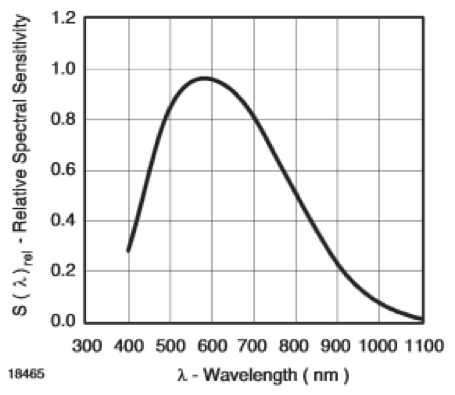
\includegraphics[height=6cm]{0_Filer/Figuer/Forudundersoegelse/TEMT6000.png}} 	
    \\ \hline
\end{tabular}
\end{table}

\begin{table}[H] \centering
\begin{tabular}{|p{3cm}|p{11cm}|}
	\hline
	\textbf{Løsning}		
	    & TSL2561 
	\\ \hline
	\textbf{Producent} 		   
	    & Texas Advanced Optoelectronic Solutions Inc. 
	\\ \hline
	\textbf{Interface} 		
	    & I2C 
	\\ \hline
	\textbf{Beskrivelse} 	
	    & Udstyret med to sensorer: En til synligt + infrarødt lys og en kun til infrarødt lys. Designet til at man tager målingen fra den første sensor og fratrækker målingen fra den anden (ligninger findes i databladet) 
	\\ \hline
	\textbf{Krav} 			
	    & Opfylder krav 1 og 2 
	\\ \hline
	\textbf{Fordele}		
	    & Burde give en fornuftig spektrum responskurve efter korrigering, bruger I2C protokol 
	\\ \hline
	\textbf{Ulemper} 		
	    & Kan ikke måle farver, kræver noget ekstra kode til korrektion 
	\\ \hline
	\textbf{Pris} 			
	    & Tilgængelig i Embedded Stock 
	\\ \hline
	\textbf{Link} 			
	    & \url{https://www.adafruit.com/datasheets/TSL2561.pdf}
	\\ \hline
	\multicolumn{2}{|c|}{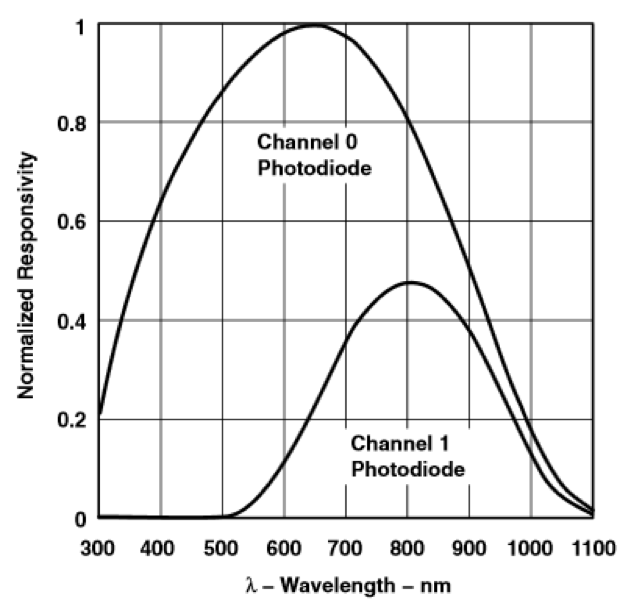
\includegraphics[height=6cm]{0_Filer/Figuer/Forudundersoegelse/TSL2561.png}} 	
    \\ \hline
\end{tabular}
\end{table}

\begin{table}[H] \centering
\begin{tabular}{|p{3cm}|p{11cm}|}
	\hline
	\textbf{Løsning}		
	    & TCS230 \\ \hline
	\textbf{Producent} 		
    	& Texas Advanced Optoelectronic Solutions Inc. 
    \\ \hline
	\textbf{Interface} 		
    	& 50\% PWM firkantsignal der ændre frekvens efter målt lysintensitet 
    \\ \hline
	\textbf{Beskrivelse} 	
    	& Udstyret med fire sensor blokke til rød, blå, grøn og hvidt (ingen filter) lys 
    \\ \hline
	\textbf{Krav} 			
    	& Opfylder krav 3 
    \\ \hline
	\textbf{Fordele}		
    	& Kan måle farver og ikke kun generel lysintensitet 
    \\ \hline
	\textbf{Ulemper} 		
	    & Har en meget dårligt spektrum responskurve, der ligger meget langt ovre i det infrarøde spektrum 
	\\ \hline
	\textbf{Pris} 			
	    & Tilgængelig i Embedded Stock 
	\\ \hline
	\textbf{Link} 			
	    & \url{http://www.pobot.org/IMG/pdf/tcs230_datasheet.pdf}
	\\ \hline
	\multicolumn{2}{|c|}{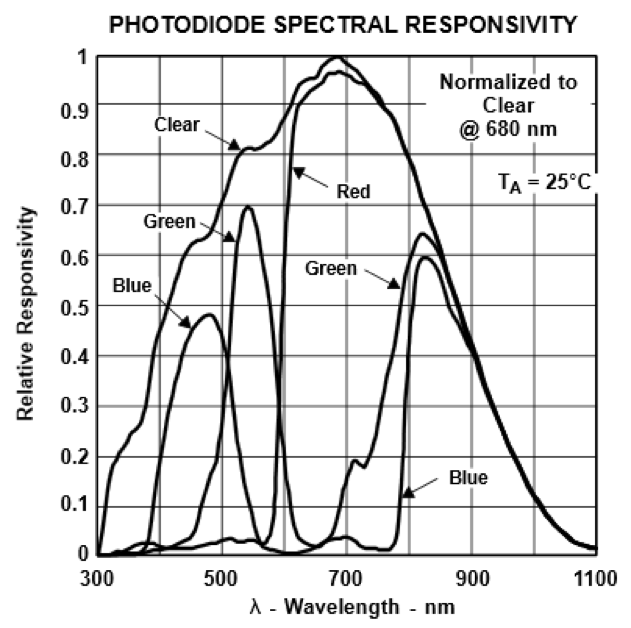
\includegraphics[height=6cm]{0_Filer/Figuer/Forudundersoegelse/TCS230.png}} 	
    \\ \hline
\end{tabular}
\end{table}

\begin{table}[H] \centering
\begin{tabular}{|p{3cm}|p{11cm}|}
	\hline
	\textbf{Løsning}		
		& TCS230 + eksternt filter (datasheet foreslåer: Hoya CM500) 
	\\ \hline
	\textbf{Producent} 		
		& Texas Advanced Optoelectronic Solutions Inc. 
	\\ \hline
	\textbf{Interface} 		
		& 50\% PWM firkantsignal der ændre frekvens efter målt lysintensitet
	\\ \hline
	\textbf{Beskrivelse} 	
		& Udstyret med fire sensor blokke til rød, blå, grøn og hvidt (ingen filter) lys 
	\\ \hline
	\textbf{Krav} 			
		& Opfylder krav 1 og 3 
	\\ \hline
	\textbf{Fordele}		
		& Kan måle farver og ikke kun generel lysintensitet. Meget god spektrum responskurve 
	\\ \hline
	\textbf{Ulemper} 		
		& Kræver indkøb af eksternt filter 
	\\ \hline
	\textbf{Pris} 			
		& Sensor: Tilgængelig i Embedded Stock. Eksternt filter: 180-190 kr. 
    \\ \hline
    \textbf{Link} 			
        & \url{http://www.pobot.org/IMG/pdf/tcs230_datasheet.pdf}
	\\ \hline
	\multicolumn{2}{|c|}{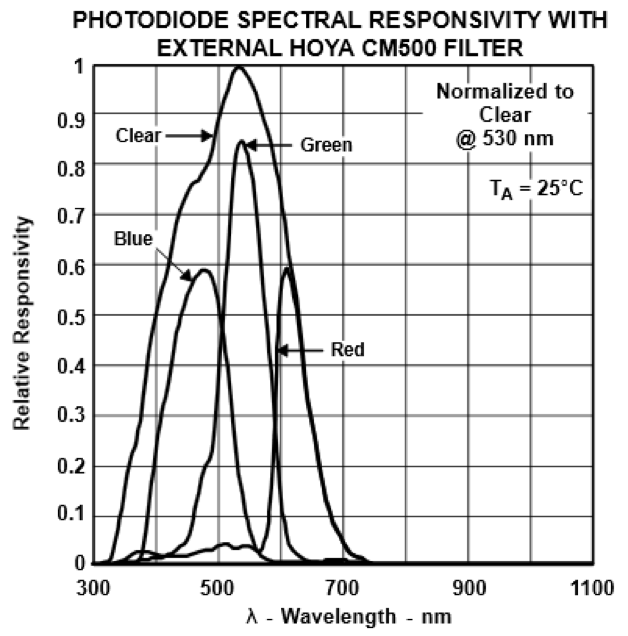
\includegraphics[height=6cm]{0_Filer/Figuer/Forudundersoegelse/TCS230-CM500.png}} 	
    \\ \hline
\end{tabular}
\end{table}

\subsection{Valg af lys sensoren}

Efter at have gennemgået databladende for alle tre sensorer, er konklusionen at arbejde videre med TSL2561 sensoren, da den umiddelbart opfylder de fleste af vores krav. Men hvis ikke kommunikationen eller differensberegningerne vil komme til at virke er TEMT6000 også en brugbar mulighed.

På den anden side, må TCS230 afvises medmindre der kan skaffes et eksternt IR filter til den.